%----------------------------------------------------------------------------------------
%	DATA ACQUISITION AND PREPARATIONS
%----------------------------------------------------------------------------------------

\section{Organization and data acquisition}
\label{ch:DataAcquisition}

In the second chapter of the report, the first stage of the study project is discussed, namely organizing, researching, and collecting the data.

The first section of the chapter~\ref{sec:Roadmap}~\nameref{sec:Roadmap} gives an overview of the time management of the study group. It is followed by the subchapter~\ref{sec:Organization}~\nameref{sec:Organization} in which communication and teamwork are assessed. In~\ref{sec:DataCollection} \nameref{sec:DataCollection}, the acquisition of the data from the sorting machine Autoselect ATS~II is described in more detail. The last section~\ref{sec:Literature}~\nameref{sec:Literature} presents the retrieved literature concerning the issue of agricultural product classification with machine learning based approaches.

\subsection{Roadmap of the project}
\label{sec:Roadmap}

At the beginning of the project, a roadmap was created to structure the year into different working stages as well as to have an overview of the tasks and problems that needed to be addressed.

\begin{figure}[h]
	\centering
	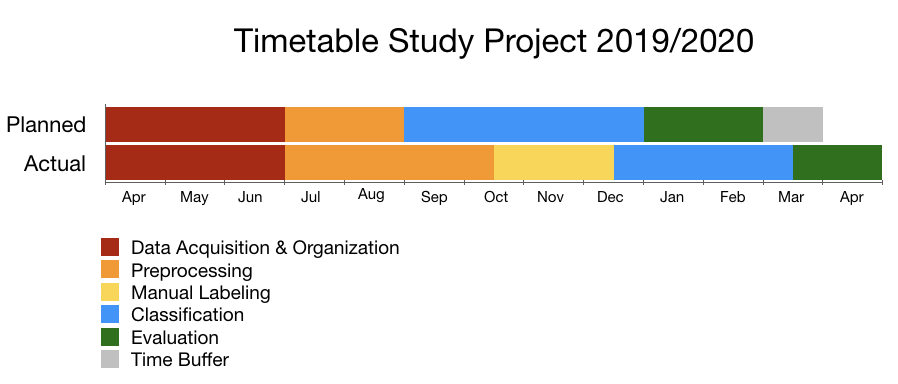
\includegraphics[scale=0.43]{Figures/chapter02/new_timetable.png}
	\decoRule
	\caption[Timetable of the Project]{\textbf{Timetable of the Project}~~~The upper timeline shows the estimated time of the study project from April 2019 to April/Mai 2020. The lower timeline displays how the time was spent. Both timelines differ in that the year was more optimistically planned than realized. Contributing factors were the lack of experience in managing a larger project and, on the technical side, the absence of expertise regarding the general implementation of the preprocessing stage. Additionally influencing the shifted timeline was the appearance of a fifth major stage, the \emph{Manual Labeling}.}
	\label{fig:Timetable}
\end{figure}

\begin{figure}[h]
	\centering
	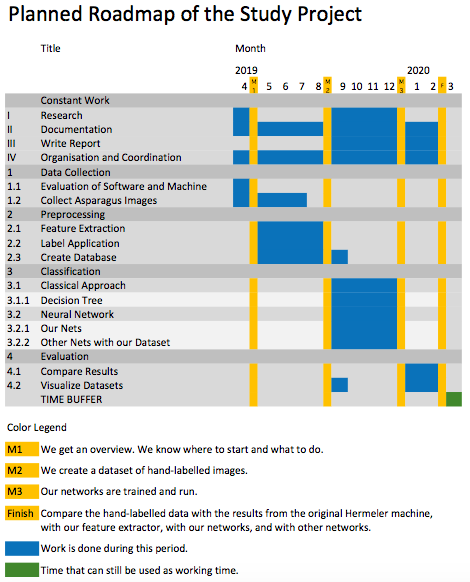
\includegraphics[scale=0.7]{Figures/chapter02/roadmap_planned.png}
	\decoRule
	\caption[Planned Roadmap]{\textbf{Planned Roadmap}~~~The figure shows the planned roadmap of the study project. It reveals how the time needed for each task was estimated in the beginning of the project.}
	\label{fig:RoadmapPlanned}
\end{figure}

\begin{figure}[h]
	\centering
	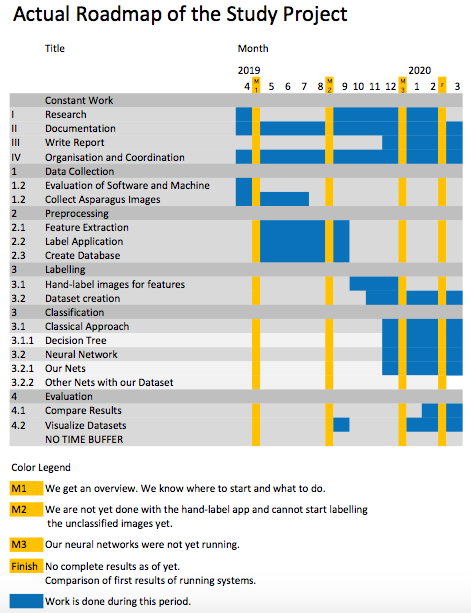
\includegraphics[scale=0.7]{Figures/chapter02/roadmap_actual.png}
	\decoRule
	\caption[Actual Roadmap]{\textbf{Actual Roadmap}~~~A roadmap that shows how the time was spent.}
	\label{fig:RoadmapActual}
\end{figure}

The timetable in~\autoref{fig:Timetable} gives a broad outline of the major stages of the project. The upper timeline of the figure shows how much time for a specific phase was estimated, whereas the lower timeline shows the real time spent on each stage. Both timelines are structured to display the project year, starting in April 2019 and ending in April/Mai 2020. The months are represented by the x-axis while the colors mark the different working stages.

The project comprises five major stages: \textit{Data Collection \& Organization}, \textit{Preprocessing}, \textit{Manual Labeling}, \textit{Classification}, and \textit{Evaluation}. A detailed representation of the single tasks attributed to each stage can be found in the roadmaps in~\autoref{fig:RoadmapPlanned} and~\autoref{fig:RoadmapActual}. The project started with the data collection. During the first stage, the images were recorded with the sorting machine, while the major planning and research for the project took place. The second phase covered the preprocessing, that is, preparing and labeling the image data. The classification stage includes the time spent on the implementation of the machine learning approaches. In the last stage, the approaches were evaluated and their results were compared. The different stages overlapped to a certain degree. For the purpose of this figure, the start and end time is displayed as a hard boundary.

It is obvious that both timelines differ. In detail, preprocessing was estimated to be done by September, however, the phase continued until October. Further, the time for labeling a sufficient amount of images was underestimated, resulting in adjustments of the time attributed to this task.

The differences are depicted with different color codings. While the main focus of this project was supposed to be the application of different machine learning techniques to classify the data (color-coded in blue and green), the preprocessing phase and the data set creation/manual labeling posed to be most time-consuming (color-coded in orange and yellow).

In~\autoref{fig:RoadmapPlanned} and~\autoref{fig:RoadmapActual}, the stage specific tasks are displayed in more detail. Again, both figures display the estimated time and the actual time, respectively. The headlines serve as a division into the major stages except for the first heading, \emph{Constant Work}, which shows the tasks that demanded continuous attention and effort throughout the year. The duration of tasks is represented in blue, while the yellow lines mark milestones that are explained in the legends.


\subsection{Organisation of the study group}
\label{sec:Organization}

This chapter focuses on the management of the work distribution and the communication. For this the used communication and organization tools will be examined as well as the structure of the group work.


\subsubsection{Communication}
\label{subsec:Communication}

The main communication took place in weekly meetings in which the working process was discussed and new tasks were distributed. In addition, different platforms were tried, which were used with varying quantities such as Asana, GitHub and Telegram. The different means of communication will be described and evaluated in the following section.

\bigskip
The weekly meetings were organized by a previously announced discussion leader and captured by a protocol writer.\footnote{The protocols were saved for review in the GitHub project at \\ \url{https://github.com/CogSciUOS/asparagus} (as of 11/27/2020)} The project’s supervisors were usually present at the meetings, to contribute with their expertise. At the beginning, tasks were distributed at the end of the meeting. In the second half of the project, the work was distributed through a schedule describing tasks and deadlines in detail. Additionally, a weekly co-working space was established. 

 Starting from the first meeting, we had a constant information exchange through a group chat on Telegram~\footnote{Telegram is a cloud-based instant messaging service for the use on smartphones, tablets and computers.}. The group chat helped to update others about the progress, support in technical issues but also created space for mutual motivation when needed.

Asana was used in the beginning of the project to distribute tasks. However, the tasks were easier to distribute in direct consultation at physical meetings and results could be easier demonstrated and discussed.

During the project, we gained a lot of expertise in using GitHub~\footnote{GitHub is a web-based popular platform using the version control system Git that helps developers to store and manage their code, and track and control changes to their project.}. Git allowed us to contribute to each other's work from anywhere, which facilitated the workflow.

Furthermore, we automatically created documentations via Sphinx. Thus, adhering to the style conventions, the protocols, work schedules, manuals, and code comments were automatically included in our documentation.\footnote{see our documentation at~\url{https://asparagus.readthedocs.io/en/latest/} (as of 11/27/2020)}


\subsubsection{Teamwork}
\label{subsec:Teamwork}

This section starts by introducing the team members and their previous experiences. It is followed by a description of the practical aspects of teamwork, the working structure, and the distribution of project-relevant tasks.

\bigskip
The project was an initiative of one member of the project group. Further students joined the project after its public announcement to complete the team.. The team was initially made up by Josefine Zerbe, Katharina Groß, Malin Spaniol, Maren Born, Michael Gerstenberger, Richard Ruppel, Sophia Schulze-Weddige, Luana Vaduva, Thomas Klein, and Subir Das. None of the members had yet worked together as such on a project of this scope. During the course of the project, three members left the team for various reasons.
The members brought a wide variety of backgrounds into the team through different bachelor programs or different majors in the broader field of Cognitive Science. In the beginning of the project, the team members had little to no experience in the application of computer vision or neural networks. The motivation of most students was to pursue new and interesting tasks in these fields. Four students had a theoretical background in computer vision, six students had gained some experience with neural networks. Git was previously only used by three students, but none of them were experts on its usage. Further, the team had neither experience with the Grid system of the \acrshort{ikw}, nor with running jobs on different machines. None of the members had prior knowledge about project management or task organization on a broader level.

\bigskip
In the beginning, the team lacked some structure and a clear distribution of individual roles. One reason for this could have been the harmonious atmosphere between team members. Further tasks such as the trips to the asparagus farm strengthened the team spirit and the social interactions. Thus, the task distribution was very dynamically structured by making every decision democratically. Most tasks were performed in smaller teams of two to three people. During meetings, tasks were formulated but not clearly assigned to members which led to a discontinuous workflow.

In August, a new structure for task distribution was introduced, such that the strengths of the individual team members could be used more efficiently. Due to the different backgrounds, team members could not resolve programming tasks equally efficiently, such that good concepts could not be realized quickly enough to include them into the project. Nevertheless, it gave the opportunity to acquire new programming skills. To integrate more of the strengths that the single team members brought and to tackle the issue of time management, it was decided to write a work schedule that distributed the work more appropriately, gave an overview of the tasks that still had to be done and showed how much time was left to do them.

The supervision of the work was divided into manager roles and the work itself into different main fields. Each member was responsible for managing their assigned area, distributing tasks and keeping an overview of the relevant work inside their working field. The manager could be consulted for questions, when in need of discussion or feedback. This distribution made the meetings more effective.

During common working hours, questions and decisions that arose could be discussed in person. This was especially helpful when different tasks overlapped and required communication and agreement.

\bigskip
In conclusion, the team structure and the distribution of work changed over the course of the project. The strengths of the single members were used more efficiently and the supervision of working areas led to a more structured time management and task distribution.


\subsection{Data collection}
\label{sec:DataCollection}

In this section the asparagus sorting machine at Gut Holsterfeld is described. Then the process of collecting labeled and unlabeled data is reported.

\begin{figure}[!t]
	\centering
	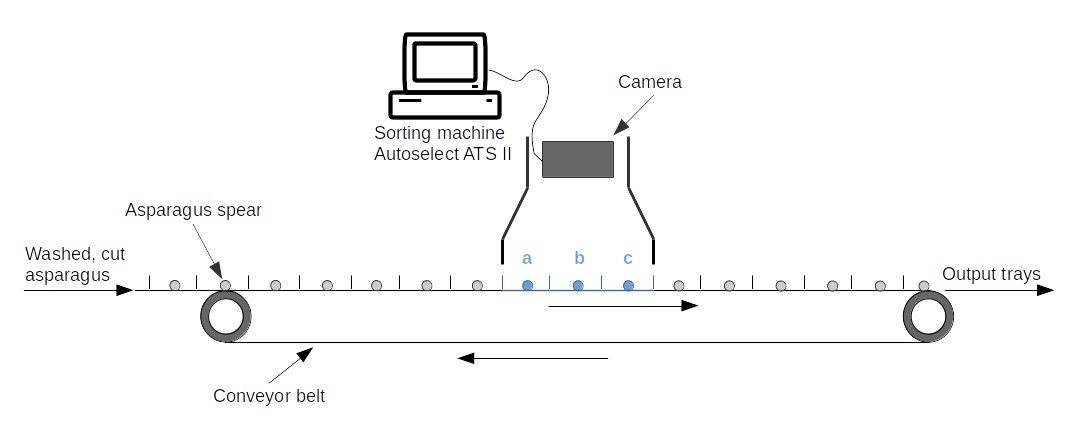
\includegraphics[width=0.9\textwidth]{Figures/chapter02/asparagusconveyerbelt_new.png}
	\decoRule
	\caption[Sketch of the Image Capturing Process with the Autoselect ATS II]{\textbf{Sketch of the Image Capturing Process with the Autoselect ATS II}~~~The asparagus spears are transported on a conveyor belt. After being washed and cut, the spears pass the camera field. Images are taken of three compartments, so that each asparagus spear is photographed three times in each position (a, b, c). The camera system is connected to a computer on which the sorting software runs. Depending on the resulting classification, the spear is sorted into the corresponding output tray.}
	\label{fig:SortingMachineSketch}
	\vspace{15pt}
	\centering
	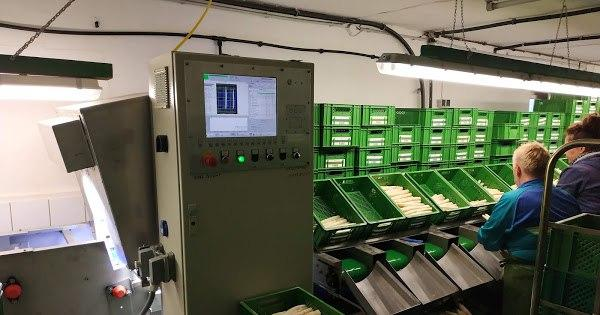
\includegraphics[scale=0.6]{Figures/chapter02/sortingmachine_front.png}
	\decoRule
	\caption[The Autoselect ATS II at Gut Holsterfeld]{\textbf{Autoselect ATS~II at Gut Holsterfeld}~~~In the figure the asparagus sorting machine Autoselect ATS~II at Gut Holsterfeld is displayed. The conveyor belt transports the asparagus from the left side of the image to the right side. It thereby passes the camera system. The display of the machine gives information on the parameters and the images. The machine is mainly controlled from here.}
	\label{fig:SortingMachine}
\end{figure}

\bigskip
The machine Autoselect ATS~II (2003) is designed for sorting white and green asparagus (see~\autoref{fig:SortingMachine}) \citep{autoselectanleitung}. First, the asparagus is arranged on a conveyor belt that runs it through the recording section of the machine. Here, a camera takes three pictures per asparagus spear (see \autoref{fig:SortingMachineSketch} and \autoref{fig:ExampleImagesAnna}). Small wheels on the conveyor belt rotate the asparagus throughout the process so that it can be photographed from several positions. In the best case, every image shows a different side of the asparagus. Subsequently, the asparagus is transported  into a tray depending on its class label. The sorting is based on the parameters for width, length, shape, curvature, rust, and color. A total of 30 criteria for classifying an asparagus spear are used to describe these parameters. The calculation of the single features is based on a classical analytical approach. For example, the parameter for color detection is composed of eight sub-parameters. Each spear is reviewed at different areas (the head of the asparagus, the area below the head, and the stem) and judged for its hue in percentage. The values are compared and, according to a threshold, the spear is sorted into a color category (e.g.\, white or violet). For all parameters, there is a minimal threshold and a maximal threshold. As another example, the parameter for width detection calculates at three points at the asparagus (top, middle, and bottom part). From these three values, an average value is calculated that decides in which category the asparagus is sorted. If an asparagus exceeds the maximal threshold for parameter detection, it is not recognized and cannot be sorted accordingly. The same holds for values below the minimal threshold. Thus, all parameters have to have an upper and a lower threshold, including parameters that decide the presence of features like shape, curvature, and color. When evaluating what parameter boundaries to choose, it is recommended to check that most asparagus spears tend to be in between the average value and the maximal threshold, with a larger tendency to accumulate around the average value. Reportedly, the parameters and their respective ranges can be freely chosen by the user and can in this way be fitted to the needs of the respective asparagus farm~\citep{autoselectanleitung}.

\begin{figure}[!htb]
	\centering
	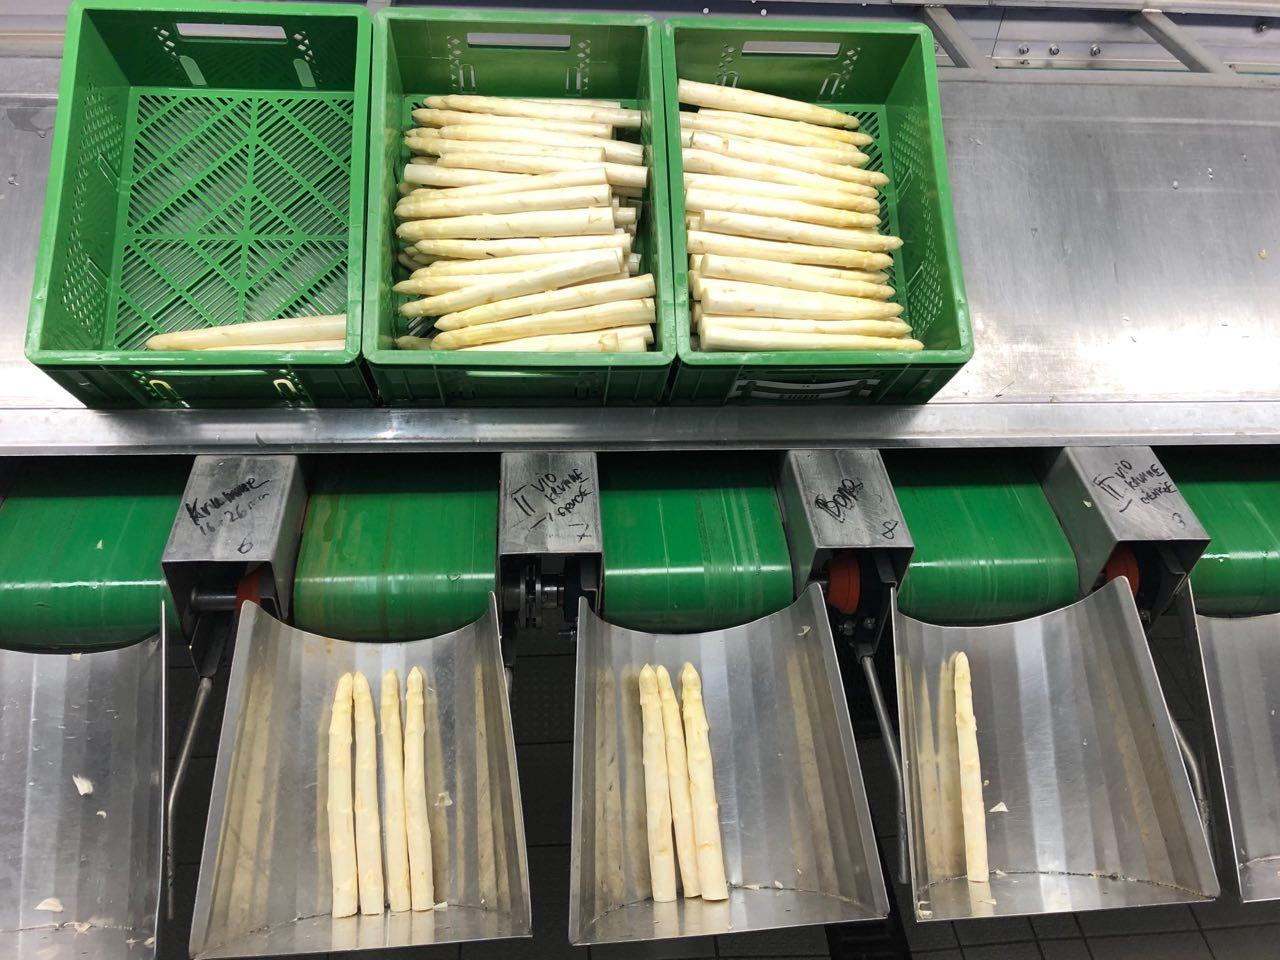
\includegraphics[scale=0.3]{Figures/chapter02/sorting_machine_slots.png}
	\decoRule
	\caption[Output Trays of the Sorting Machine]{\textbf{Output Trays of the Sorting Machine}~~~Depending on the class label, the asparagus is sorted into one of the machine's 16 trays.}
	\label{fig:SortingMachineSlots}
\end{figure}

Before the first use of the machine, all parameters are selected after a calibrating charge of asparagus has run through the machine. Then, the user can adjust the thresholds accordingly.

According to the manual, the number of quality classes is selectable, by choosing the arrangement of parameters. The manufacturer suggests to first sort for length and width, then use the parameters that sort for color, and the parameters for shape detection last.

The accuracy of the sorting machine is described to be as good as 90\% best case by the manufacturer, while the farmer at Gut Holsterfeld reported it to be around 70\% at best, with re-sorting being necessary by professional sorters. Especially categories like Blume or Hohle were considered to be inconsistent by both, manufacturer and farmer. Further information could not be given on the software of the machine. A meeting with a representative of the engineering company HMF~\footnote{see \url{www.hmf-hermeler.de} (visited on 03/15/2020)}  that manufactured the sorting machine was arranged. Unfortunately, the source code itself was not available to HMF as it was produced by another company. 

\bigskip
It is possible to save images with the Autoselect ATS II, however, the storage space on the machine is very limited. Further, the selection of images to be saved is restricted to only 1000 images at a time.
One workaround to the problem is the installation of the Teamviewer software~\footnote{see \url{https://www.teamviewer.com/en/} (visited on 03/15/2020)} on the machine and the connection of an external hard drive. After the installation, the process of image collection could be started remotely. This work was very ineffective and time-consuming. The data could not be directly transmitted to another computer because of the lack of internet speed at the farm. An automatic transfer of the images to the external hard drive was not possible until the installation of an automatic file moving service, for which the requirements are described below.

The file moving program transfers the images to a new saving destination and runs in the background without disturbing the workflow of the sorting machine. We decided to use a service, that is, a system process running independently of any program. The service manages moving the newly generated image files, as described in detail in the appendix in \autoref{subsec:FileService}.

Hard drives were collected two times a week to subsequently store the collected images in the storage capacities of the university.

The label that the machine attributes to each asparagus is not reliable. Therefore, sending the asparagus through the machine a second time would be the only way to gather labeled images. Unfortunately, a second sorting degrades the quality of the asparagus. Therefore, only a limited amount of labeled data was collected. 

\begin{figure}[!h]
	\centering
	\vspace{20pt}
	\begin{subfigure}{0.3\textwidth}
		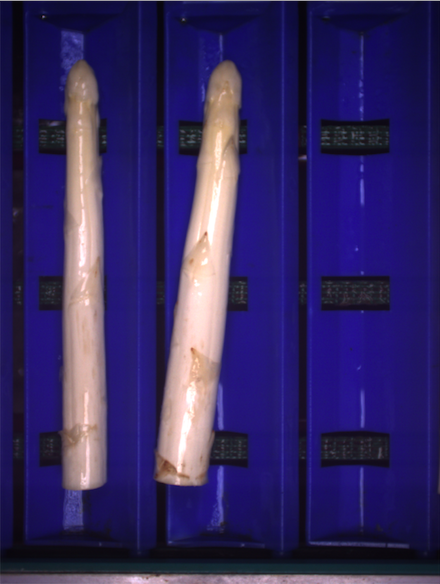
\includegraphics[width=0.95\linewidth]{Figures/chapter02/anna_a.png}
		\caption{left}
	\end{subfigure}
	\begin{subfigure}{0.3\textwidth}
		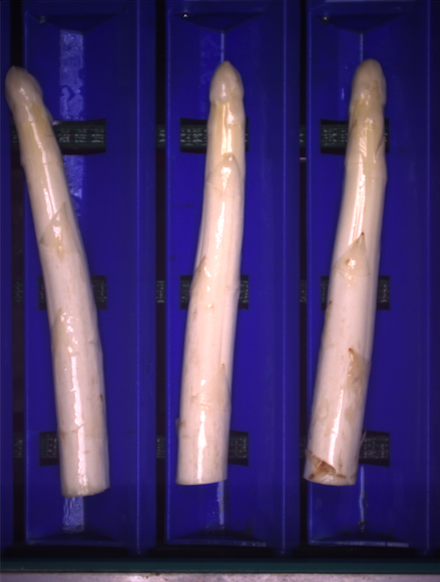
\includegraphics[width=0.95\linewidth]{Figures/chapter02/anna_b.png}
		\caption{middle}
	\end{subfigure}
	\begin{subfigure}{0.3\textwidth}
		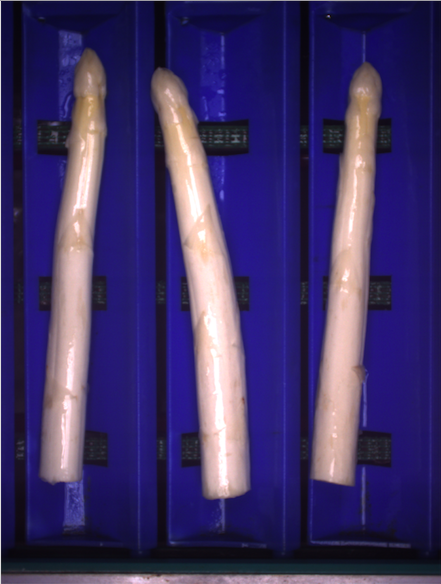
\includegraphics[width=0.95\linewidth]{Figures/chapter02/anna_c.png}
		\caption{right}
	\end{subfigure}
    \caption[Example Asparagus Images]{\textbf{Example Asparagus Images}~~~Example pictures of the quality class I~A~Anna whose capturing process is described in \autoref{fig:SortingMachineSketch}. In picture (A) the target asparagus is to the left, in (B) it is in the middle, and in (C) it is to the right. Small wheels on the conveyor belt rotate the asparagus in the meantime so that it can be photographed from several positions. 
}
    \label{fig:ExampleImagesAnna}
\end{figure}

An example image of the received data can be seen in~\autoref{fig:ExampleImagesAnna}. There are three pictures per asparagus. The image resolution is $1040\times1376$ pixel per image, with an RGB color space.

\begin{table}[!htb]
	\centering
	\resizebox{.95\linewidth}{!}{%
	\begin{tabular}{|lr|lr|lr|}
		\hline
		\textbf{Class Label~~~~~} & \textbf{Nr. of Images} & \textbf{Class Label~~~~~} & \textbf{Nr. of Images} & \textbf{Class Label~~~~~} & \textbf{Nr. of Images} \\
		\hline
		I~A Anna		& 1005	& II~A	& 1051 	& Blume	& 1717	\\
		I~A Bona		& 908 	& II~B 	& 1468 	& Suppe	& 1157	\\
		I~A Clara	& 513 	& Rost 	& 1169	& Bruch	& 309	\\
		I~A Krumme	& 936 	& Dicke & 749 	& {}		& {}		\\
		I~A Violett	& 1514 	& Hohle	& 775 	& {}		& {}		\\
		\hline
	\end{tabular}%
	}
	\caption[Collected Images with Class Label]{\textbf{Collected Images with Class Label} \\ In this table, the number of collected images with a class label is reported. This was achieved by running pre-sorted spears through the sorting machine a second time.}
	\label{tab:LabeledClassNumber}
\end{table}

\begin{figure}[!ht]
	\centering
	\vspace{20pt}
	\begin{subfigure}{0.3\textwidth}
		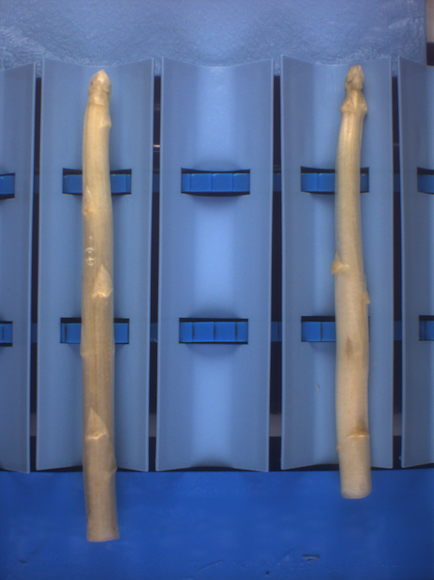
\includegraphics[width=0.9\linewidth]{Figures/chapter02/querdel_a.png}
		\caption{left}
	\end{subfigure}
	\begin{subfigure}{0.3\textwidth}
		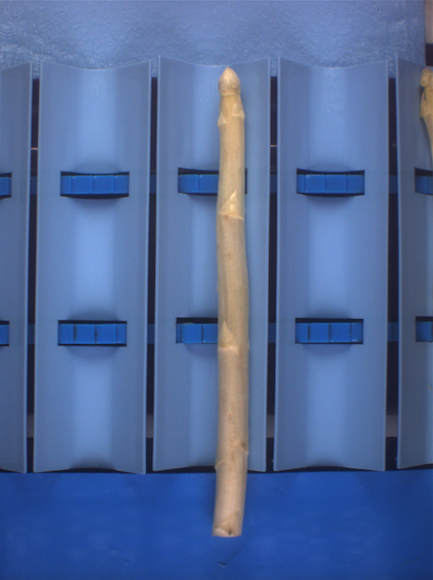
\includegraphics[width=0.9\linewidth]{Figures/chapter02/querdel_b.png}
		\caption{middle}
	\end{subfigure}
	\begin{subfigure}{0.3\textwidth}
		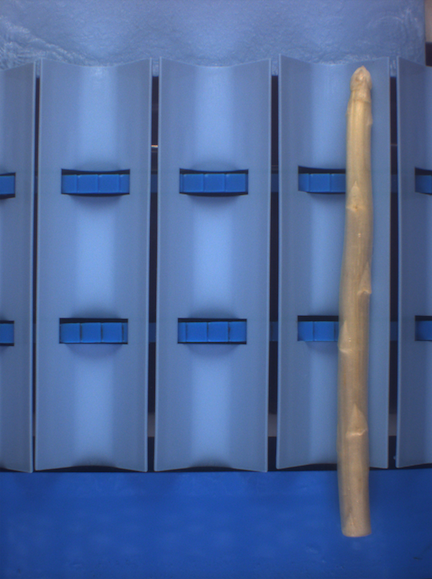
\includegraphics[width=0.9\linewidth]{Figures/chapter02/querdel_c.png}
		\caption{right}
	\end{subfigure}
	
	\begin{subfigure}{0.3\textwidth}
		\vspace{10pt}
		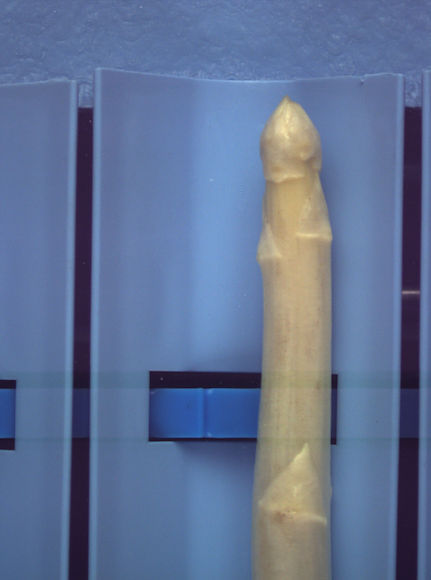
\includegraphics[width=0.9\linewidth]{Figures/chapter02/querdel_d.png}
		\caption{upper part}
	\end{subfigure}
    \caption[Example Asparagus Images Querdel's Hof]{\textbf{Example Images Querdel's Hof}~~~Example pictures of the asparagus of the farm Querdel's Hof. In picture (A), the asparagus spear is to the left, in (B), it is in the middle, and in (C) it is to the right. A fourth picture (D) is taken with a second camera with focus on the upper part of the asparagus.}
    \label{fig:ExampleImagesQuerdel}
\end{figure}

\bigskip
In total, 612113 images were collected, with each class label being represented with at least 309 images, corresponding to 103 asparagus.

At the asparagus farm Gut Holsterfeld, 591495 labeled and unlabeled images were collected with the Autoselect ATS~II. The number of unlabeled data is 578226 images, thus, around 192742 different asparagus spears. Of the labeled data, the number of images that were collected per quality class can be found in \autoref{tab:LabeledClassNumber}. The image number does not represent the number of different asparagus spears, as each asparagus spear is represented by three distinct images.

Additionally, a few images could be recorded at another asparagus farm, Querdel’s Hof~\footnote{see~\url{https://www.querdel.de/} (visited on 03/15/2020)}, in Emsb{\"u}ren. The farm sorts the asparagus with an updated version of the Autoselect ATS~II at Gut Holsterfeld, that is, it uses the same software but other hardware. In particular the resolution of the camera was improved and a second camera focuses on the head region of the asparagus. At Querdel’s Hof, 20616 images were collected in total, 76 from the class label \enquote{normal}, 152 from the class label \enquote{violet/flower}, and 20388 unlabeled images. Each asparagus spear is represented by four images: three images show the asparagus from different perspectives and a fourth image depicts solely the head region. Example images for one asparagus can be seen in~\autoref{fig:ExampleImagesQuerdel}. No internet connection could be established on the farm, thus, no further images were collected. Moreover, the data format of the images from Querdel’s Hof is different to the data from the farm Gut Holsterfeld. Therefore a combination of both data sets was inconvenient.


\subsection{Literature on food classification using computer vision}
\label{sec:Literature}

In the classification of food products, there are numerous possibilities to apply machine learning approaches for classification tasks on image data~\citep{bhargava2018fruits,brosnan2002inspection}.


For the scope of this investigation, we decided to focus our literature search on fruit and vegetable quality evaluation using computer vision and machine learning. Compared to other fields, research and evaluation in agricultural classification shares many characteristics and faces similar difficulties.

The quality inspection based on computer vision is usually constituted into five main steps: image acquisition, preprocessing, image segmentation, feature extraction and classification~\citep{bhargava2018fruits}. Moreover, most data in agriculture is based on photographic images. Also the features of interest are similar for different kinds of fruit or vegetable. Features that are frequently inspected by traditional computer vision techniques concern color, shape, size, texture, and defect~\citep{bhargava2018fruits}. This makes other papers in the field of agricultural evaluation directly comparable to our case. Moreover, we hope to get an impression of the state of the art of how many images are needed in our case, how high the image resolution needs to be, what kind of computer vision approaches could be helpful as a starting point, and also to become aware of known challenges.

\bigskip
None of the found papers were suitable as blueprints for the asparagus classification project. However, some of them helped to get an idea of how to proceed with the project. For example, some papers show how the preprocessing phase could be structured~\citep{mery2013automated}, or they evaluate the machine learning methods that were already used on other food classification tasks~\citep{bhargava2018fruits}. Further, some of the literature is concerned with the classification of food products but not with differentiating between as many classes as 13~\citep{diaz2004comparison,kilicc2007classification}. Often, the variance in the food products, that is, the quality as well as the type of food used is either too high~\citep{zhang2012classification} or too low~\citep{kilicc2007classification,al2011dates} in comparison to the variance in our project data. One paper evaluates the sorting of asparagus, however, it only does so on a small data set with three categories of green asparagus~\citep{donis2016classification}. Further papers on food classification are not detailed enough in their explanations and do not share the information needed for replication~\citep{pedreschi2016grading}.

Even though no specific paper was used as guidance to our project, some specific papers inspired us to try out certain algorithms, such as \acrshort{pca} ~\citep{Vijayarekha2008, Zhu2007}) or neural networks ~\citep{Jhuria2013, Pujari2014}. Moreover, the literature review made us aware of the limiting fact that images of fruits and vegetables are captured mainly from one direction~\citep{bhargava2018fruits}.The literature suggests that performance might improve, if more perspectives are taken into account. Moreover, the literature shows that different authors use different color spaces such as CIE Lab, RGB or HSI ~\citep{Liming2010, Garrido-Novell2012, Kondo2010}. This further inspired us to apply color quantization on our data.

\bigbreak
As the available data was only sparsely labeled, further research was done to evaluate the use of a semi-supervised learning approach~\citep{olivier2006semi,zhu05survey}. Details about the corresponding literature can be found in~\autoref{sec:SemiSupervisedLearning}. In regards to deep learning-based approaches, classical neural networks -- such as AlexNet \citep{alexnet2012original}, \acrshort{vgg}16/\acrshort{vgg}19 \citep{vgg2014original}, GoogleNet \citep{googlenet2015original}, Capsule Networks \citep{capsulenet2017original},  DenseNet \citep{densenet2017original}, ResNet \citep{resnet2016original} or \acrfull{nin} \citep{lin2013network} -- were assessed for better understanding of the range of possible pre-trained networks and ideas for network structures. Additonal machine learning approaches were considered, like multiclass \acrfullpl{svm} \citep{prakash2012multi}.
